\subsection{Thiết kế thử nghiệm cải thiện RUL}
\label{sec:rul-improvement-method}

Thực nghiệm bổ sung kiểm tra ba giả thuyết: window ngắn hơn có thể theo sát
thay đổi gần thời điểm hỏng; chỉnh tham số có thể giảm sai số; tăng trọng số
cho mẫu RUL thấp có thể cải thiện dự đoán ở cuối vòng đời. Thực nghiệm giữ
HistGradientBoostingRegressor, target RUL gốc và 126 đặc trưng hiện có.
Các giả thuyết không bảo đảm kết quả tốt hơn baseline.

Nested GroupKFold gồm 5 vòng ngoài và 3 vòng trong, tất cả chia theo engine
\cite{sklearnNestedCV2026,sklearnGroupedCV}.
Outer assignments lấy từ lần đánh giá baseline. Trong mỗi vòng ngoài, engine
validation không tham gia fit hoặc chọn cấu hình. Inner CV chỉ dùng engine
thuộc outer train. Ba window 10, 20 và 30 cùng dùng 17.731 khóa từ cycle 30
trở đi. Cách này giữ nguyên số dòng so sánh, chỉ thay số cycle quá khứ dùng
để tính đặc trưng. Window 50 không được xét vì 7 test engines có ít hơn 50
observations, trong khi contract hiện tại yêu cầu window đủ dài.

Sau bước chọn window, 24 cấu hình HGB được đánh giá: cấu hình gốc và 23 cấu
hình khác nhau lấy mẫu bằng seed 42. Các giá trị gồm learning rate
$\{0{,}03;0{,}05;0{,}1\}$, số vòng boosting $\{100;200;400\}$, số lá tối đa
$\{15;31;63\}$, số mẫu tối thiểu tại lá $\{10;20;40\}$ và L2
$\{0;0{,}01;0{,}1\}$. Giữ \texttt{early\_stopping=False} để tránh một phép
chia ngẫu nhiên theo dòng trong quá trình fit \cite{sklearnHGBAPI2026}.

Ba phương án trọng số lần lượt dùng hệ số $(1;1;1)$, $(1;1{,}5;2)$ và
$(1;2;3)$ cho các vùng $\mathrm{RUL}>30$, $15<\mathrm{RUL}\leq30$ và
$\mathrm{RUL}\leq15$. Với từng engine, chia hệ số của mỗi dòng cho tổng hệ số
của engine đó, nên tổng trọng số mỗi engine bằng 1. Ví dụ hai dòng có hệ số
1 và 3 nhận trọng số 0,25 và 0,75. Metric đánh giá giữ nguyên, không áp dụng
trọng số ưu tiên mẫu RUL thấp.

Metric chính khi chọn cấu hình là MAE ở vùng RUL không quá 30, tính trong
từng engine rồi lấy trung bình. Ứng viên hợp lệ phải đồng thời không tăng
MAE toàn bộ, tỷ lệ cảnh báo sau mốc RUL thật bằng 30 hoặc bỏ lỡ, và tỷ lệ thời
gian báo sớm so với baseline của giai đoạn. Tỷ lệ thời gian báo sớm là tỷ lệ
dòng có $\widehat{\mathrm{RUL}}\leq30$ trong vùng $\mathrm{RUL}>30$, tính theo
engine rồi lấy trung bình. Đại lượng này khác tỷ lệ cảnh báo sai cấp engine
trên toàn vòng đời. Khi hòa metric chính, thứ tự ưu tiên là tỷ lệ cảnh báo
trễ hoặc bỏ lỡ, MAE toàn bộ, rồi candidate ID cố định.

Outer predictions được lưu cho baseline và phương án được chọn ở cuối mỗi
giai đoạn. Paired bootstrap lấy lại cùng engine IDs cho hai phương án,
10.000 lần với seed 42. Khoảng tin cậy phản ánh độ bất định trên predictions
đã tạo; chưa bao gồm biến thiên nếu huấn luyện lại. Cấu hình cuối được chọn
bằng đúng quy trình inner CV trên toàn bộ train, sau đó fit lại. Nhãn test
chỉ được ghép sau khi ghi 100 predictions. Test FD001 đã được xem trong các
phân tích trước đợt này, kể cả lượt kiểm tra runner ban đầu; đóng test trong
search mới không xóa lịch sử đó.

\begin{figure}[H]
\centering
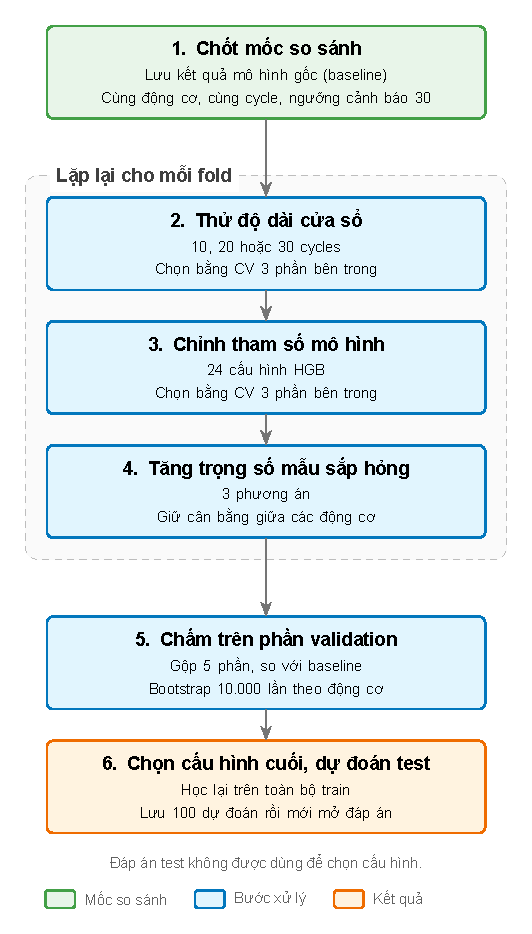
\includegraphics[width=0.86\textwidth]{figures/rul-improvement.pdf}
\caption{Quy trình chọn cấu hình và đánh giá ngoài theo engine. Các bước chọn window, tham số và trọng số đều nằm trong inner CV.}
\label{fig:rul-improvement}
\end{figure}
